% !TEX root = main.tex
\documentclass[a4paper, UKenglish, 11pt]{uiomaster}
\usepackage{lipsum}
\usepackage[subpreambles=true]{standalone}
\usepackage[table,xcdraw]{xcolor}

\begin{document}
\chapter{Convolutional Neural Network Approach for Localizing Single Dipole Sources}
In this chapter, we explore the utilization of a Convolutional Neural Network (CNN) for the task of localizing simple current dipoles from EEG recordings. The CNN is a sophisticated type of feed-forward neural network that excels at learning spatial features from images. The objective of this investigation is to assess whether leveraging spatial information in EEG recordings as images can enhance Dilocs's ability to analyze the data and yield more accurate predictions for localizing the sources generating the neural signals.

\subsubsection{Convolutional Neural Networks}
Convolutional neural networks (CNNs) is an other variant of FFNNs that have drawen inspiration from the functioning of the visual cortex of the brain. In the visual cortex, individual neurons exhibit selective responses to stimuli within small sub-regions of the visual field, known as receptive fields. This property allows the neurons to effectively exploit the spatially local correlations present in natural images. Mathematically, the response of each neuron can be approximated using a convolution operation \cite{Hjorth-Jensen2022}.

% TODO: check sources
CNNs mimic the behavior of visual cortex neurons by utializing a specific connectivity pattern between nodes in adjacent layers. Unlike fully contected FFNNs, where each node connects to all nodes in the preceding layer, CNNs  local connectivity. In other words, each node in a convolutional layer is only connected to a subset of nodes in the previous layer. Typically, CNNs consist of multiple convolutional layers that learn local features from the input data. These layers are followed by a fully connected layer that combines the learned local information to produce the final outputs. CNNs find wide applications in image and video recognition tasks \cite{Hjorth-Jensen2022}.



\subsection{Data Set}

Convolutional Neural Networks (CNNs) are well-known for their effectiveness in processing image data. To harness the potential of CNNs for EEG data analysis, we convert the original dataset presented in Chapter 4 into image-like data through interpolation. Interpolation, a widely-used mathematical technique, estimates values between known data points. This transformation results in a regular 2D grid representation of the original one-dimensional EEG data, effectively creating EEG data with image-like characteristics and preserving spatial structures.

The resulting data is represented as a 20x20 matrix, where each element holds the intensity value of the EEG potential recorded at the corresponding electrode location. We construct this matrix to resemble the shape of a grayscale image, with a single channel added to represent the spatial distribution of the measured EEG signals. However, unlike typical grayscale images where each pixel represents color intensity, in this context, each pixel's value denotes the intensity of the recorded EEG signal at that specific electrode location. This unique representation enables the CNN to leverage the spatial arrangement of the EEG data and learn relevant patterns and local relationships, much like how CNNs process traditional image data.

The preserved spatial structures enable the network to exploit local relationships between neighboring recording electrodes. For instance, when neighboring electrodes record high EEG values, it suggests that the specific electrode should also record a relatively high EEG value due to their close spatial proximity. These spatial relationships may contribute to faster training times for the network, as it can efficiently learn meaningful representations by leveraging these patterns.

Figure \ref{ref:eeg_dipole_pos_0} illustrates the process of interpolation. The right panel shows the original data, representing the cortex seen from above (x-y-plane). Each measuring electrode is depicted as a circle holding the EEG recording at that specific electrode. The middle and left panels display the contour plots of the original EEG data and the interpolated data, respectively. The contour plot of the interpolated data illustrates how the input data for the convolutional neural network appears in an image-like manner.


\begin{figure}[!htb]
\centering
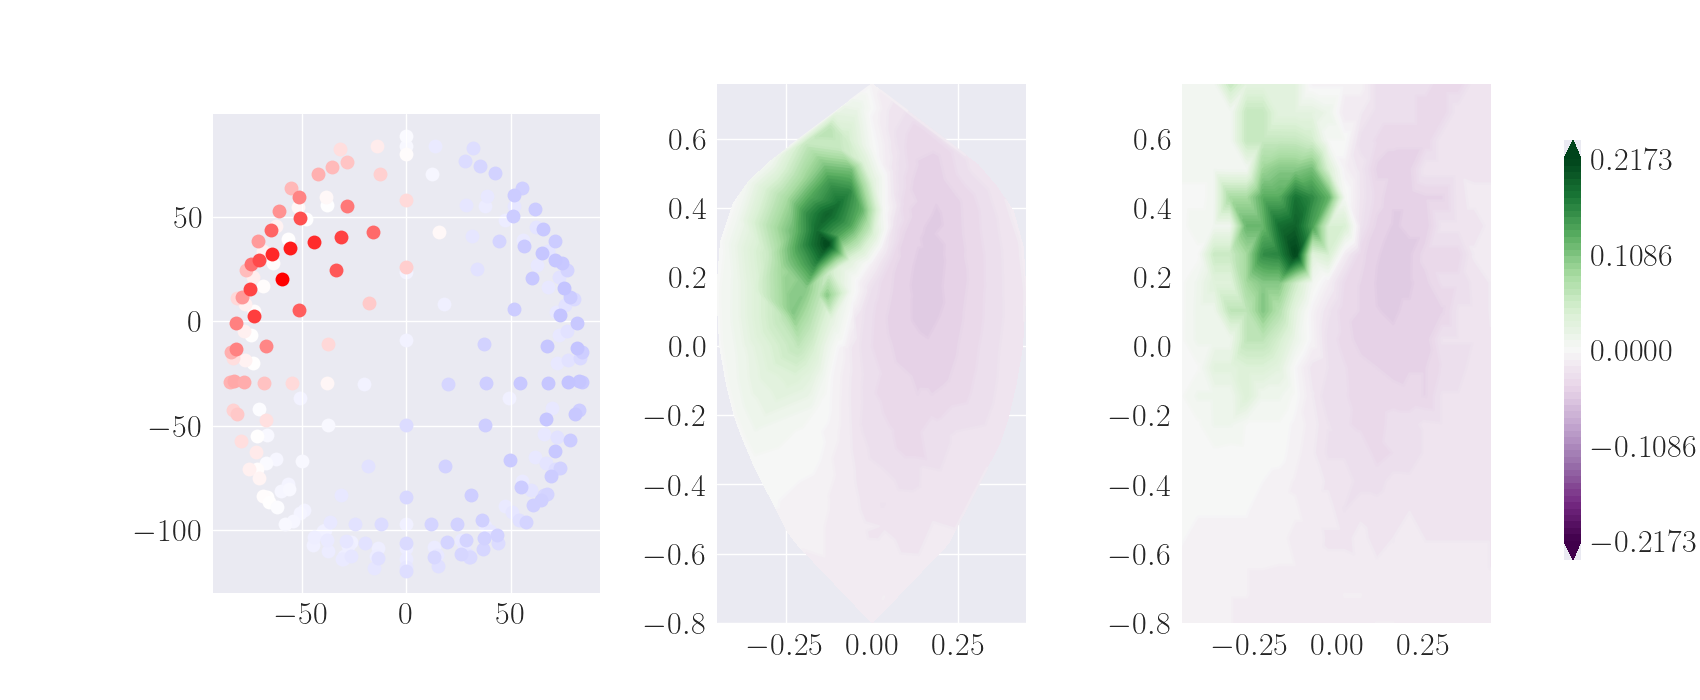
\includegraphics[width=\linewidth]{../Code/plots/finals/new_eeg_dipole_pos_0.png}
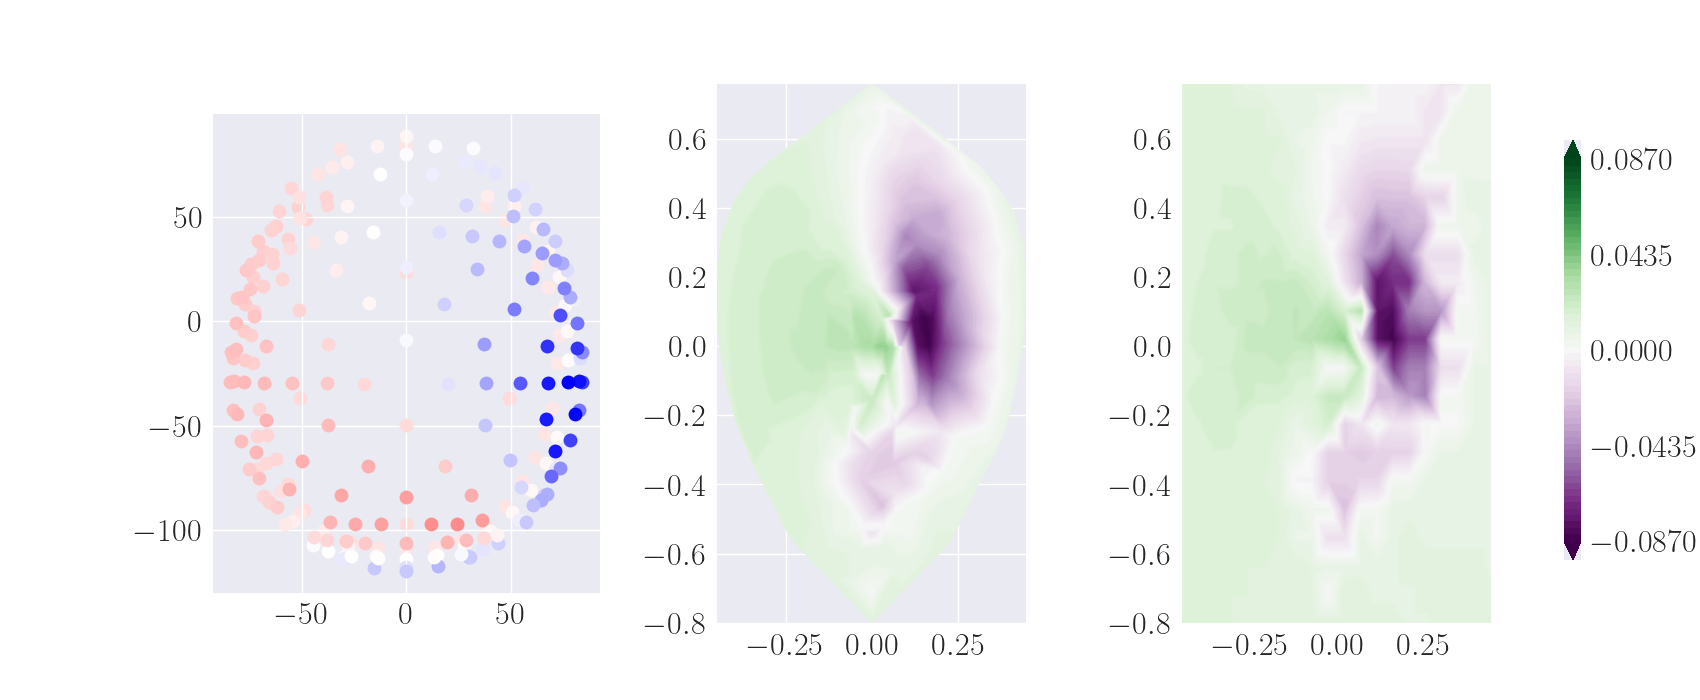
\includegraphics[width=\linewidth]{../Code/plots/finals/new_eeg_dipole_pos_4.png}
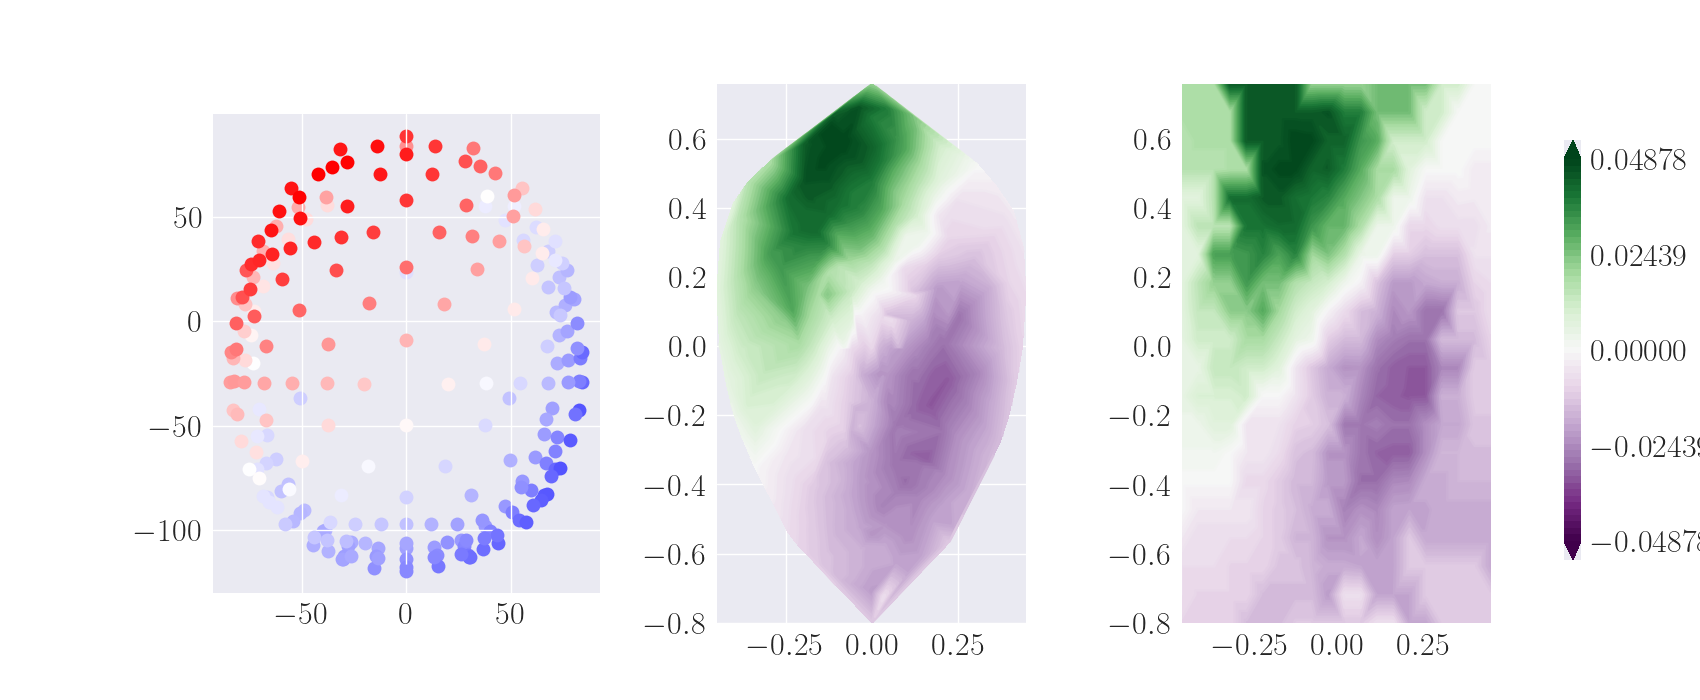
\includegraphics[width=\linewidth]{../Code/plots/finals/new_eeg_dipole_pos_6.png}

\caption{\newline
\textbf{Right Panel:} EEG measures for three different samples, expressed in microvolts ($\mu V$). Each sample represents an EEG recording at specific electrode positions. \newline
\textbf{Middle and Left Panels:} Illustration of the interpolation of the EEG data into a two-dimensional matrix. The interpolated data represents the transformation of original electrode recordings into a regular 2D grid, effectively converting the one-dimensional EEG data into an image-like format. The contour plots visualize the spatial distribution of EEG potential intensities, with each point in the matrix corresponding to a specific electrode location.}
\label{fig:eeg_dipole_pos_0}

\end{figure}

\subsubsection{Architecture, Hyperparameters and Training}

% REWRITE; FIND SOURCES OF WHAT EACH LAYER DOES (this is not your work)
As explained in Chapter 3, Convolutional Neural Networks (CNNs) are structured as a sequence of interconnected layers designed to process and extract meaningful features from the input data. In the case of EEG input data, we adopt a specialized CNN architecture tailored to handle image-like data representations. The data transformation involves constructing a 20x20 matrix, akin to the shape of a grayscale image, with a single channel added to represent the spatial distribution of the measured EEG signals.

The first layer in the network, is a 2D convolutional layer. It takes the input image with one channel and applies six distinct filters, each of size 5x5. These filters are responsible for learning specific spatial patterns and detecting relevant features within the input image. As a result of this convolutional operation, the output tensor's spatial dimensions reduce to 16x16, and the depth becomes six, signifying the extraction of six distinct feature maps. Following the convolution layer, a Max Pooling layer, with kernal size 2x2 and stride 1 is employed. This pooling layer aims to downsample the spatial dimensions of the feature maps while preserving the most salient features. The pooling operation reduces the spatial resolution to 15x15, and the depth remains unchanged at six. Next, a second 2D convolutional layer, takes the six-channel output from the previous pooling layer. This layer employs 16 filters of size 5x5, extracting a more complex hierarchy of features from the input data. The output tensor from this layer has spatial dimensions of 11x11 and a depth of 16, signifying the presence of 16 distinct feature maps. Following another Max Pooling layer is employed. Similar to the previous pooling operation, this layer further downsamples the spatial dimensions while preserving the depth, resulting in a feature map size of 10x10 with 16 channels. Further, the output from the last pooling layer is flattened into a one-dimensional vector. This process collapses the spatial dimensions of the feature maps, resulting in a 1D tensor of size 1600 (10x10x16). After flattening, the network proceeds with three fully connected, dense, layers. These layers are responsible for incorporating global context and making high-level abstractions from the learned features. The first fully connected layer, consists of 120 neurons, followed by 64 neurons. Lastly,we have the output layer with three neurons, corresponding to the three coordinates of the source generating the eeg signal. In Figure \ref{fig:architecture_CNN}, we have provided an illusration of the architecture of the Convolutional Neural Network.

The activation function ReLU is applied after each convolutional and pooling layer, introducing non-linearity to the network and enabling it to learn complex relationships within the data. The fully connected layers use the hyperbolic tangent activation function, which introduces non-linearity and scales the output between -1 and 1. Finally, in the output layer, we opted for a linear transformation without the use of any activation function. This setup allows the neural network to provide direct and unconstrained predictions for the x-, y-, and z-positions of the desired dipole source, as required in our application.Throughout the network, the weights of the fully connected layers are initialized using the Xavier normal distribution, a widely used technique to set initial weights in deep neural networks, promoting better convergence during training.

% On later point, discuss how batch size = 64 might have led to less loiser convergence.
The training process for the specialized convolutional neural network (CNN) followed similar techniques to the original DiLoc network, as described in detail in Chapter 5. To ensure effective learning and accurate predictions, stochastic gradient descent (SGD) with momentum was utilized as the optimizer, and mean squared error (MSE) served as the chosen cost function. Additionally, L1 and L2 regularization techniques were incorporated to mitigate overfitting and enhance the network's ability to generalize to new data. During training, mini-batches of size 32 were employed to introduce variability in the data and prevent the network from becoming stuck in local minima. Notably, the CNN employed specific hyperparameters, setting the learning rate to 0.001 and the momentum to 0.009, which were tailored to accommodate the processing requirements of image-like EEG data. To facilitate convergence, a learning rate scheduling approach was adopted, gradually reducing the learning rate during training, striking a balance between rapid initial convergence and fine-tuning towards the later stages. Subsequently, the CNN's performance was rigorously evaluated on an independent test dataset to provide an unbiased assessment of its predictive accuracy and generalization capabilities to novel data.

\begin{figure}[!htb]
    \hspace*{-3cm} % Adjust the value here to move the figure more to the left
    \centering
    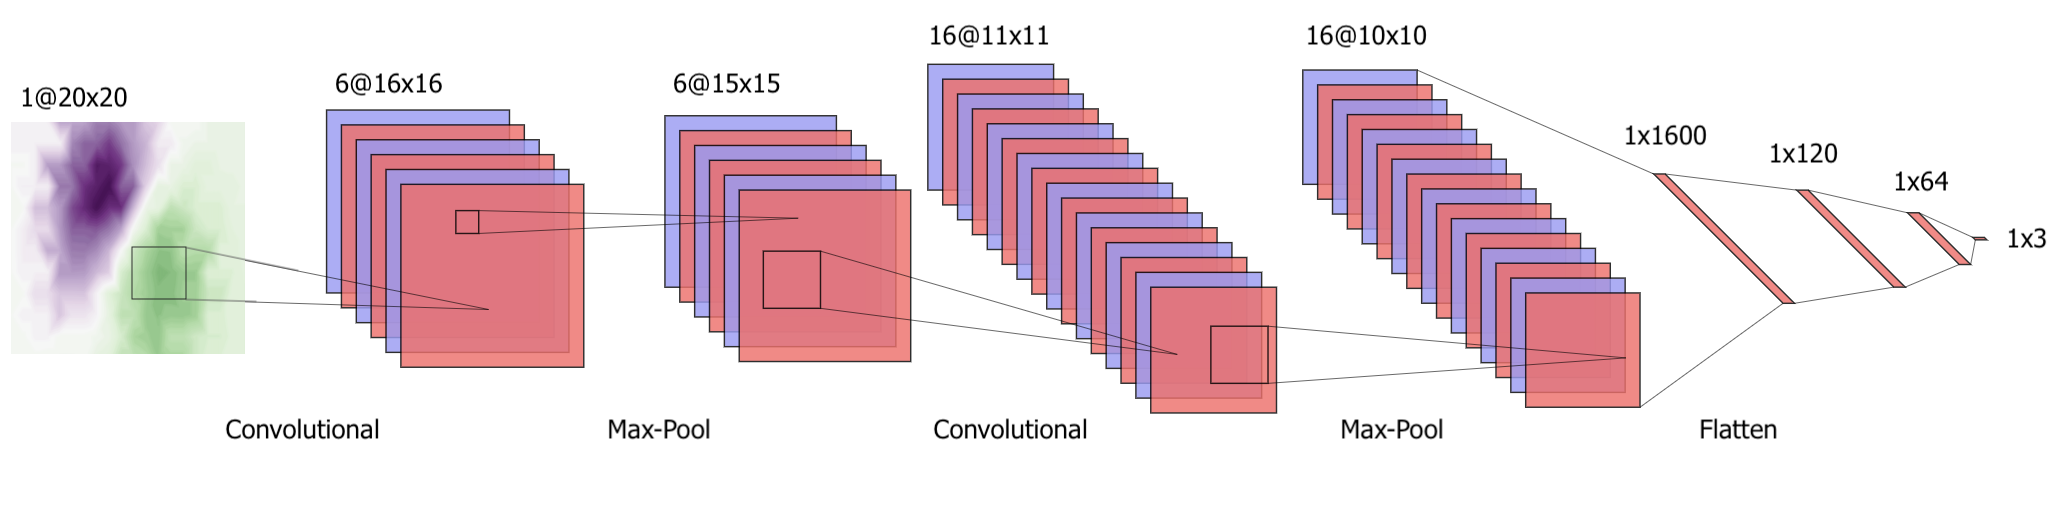
\includegraphics[scale=0.52]{figures/CNN.png}
    \caption{The architecture of the Convolutional Neural Network.}
    \label{fig:architecture_CNN}
\end{figure}


\subsection{Performance Evaluation}

\begin{figure}[!htb]
    \centering
    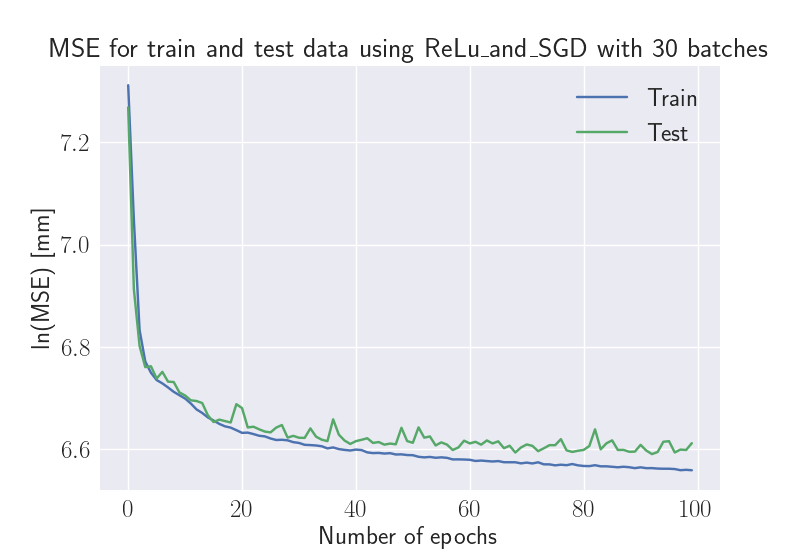
\includegraphics[width=\linewidth]{../Code/plots/finals/MSE_CNN_dipoles_2_interpolated_CNN_20x20_10000_ReLu_and_SGD_30_100.png}
    \caption{The validation accuracy for Convolutional Neural Network with 10 000 samples (20x20 matrix) with ReLU activation function. }
    \label{fig:single_dipole_accuracy_CNN_2d}
\end{figure}

% \begin{figure}[!htb]
%     \centering
%     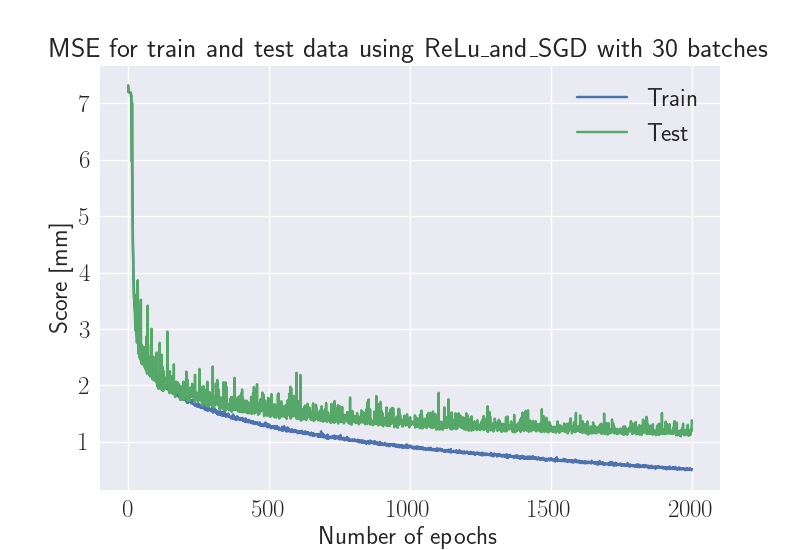
\includegraphics[width=\linewidth]{../Code/plots/CNN/MSE_interpolated_CNN_20x20_10000_ReLu_and_SGD_30_2000.png}
%     \caption{The validation accuracy for Convolutional Neural Network with 10 000 samples (20x20 interpolated matrix) with ReLU activation function. }
%     \label{fig:single_dipole_accuracy_CNN}
% \end{figure}

\end{document}